\documentclass[12pt, a4paper]{article} % default font size, paper size, document type
\title{Latex Cheatsheet}
\usepackage{graphicx} %  allows for images
\usepackage{amsmath}
\usepackage[utf8]{inputenc}
\usepackage[T1]{fontenc}
\graphicspath{{images/}} % specifies directory with images
\author{Wiktor Zajac}
\date{October 2023}
\begin{document}

\maketitle
\vspace{5mm}

\section{Random}

\textbf{bold text}

\textit{italic text}

\underline{underline}

\emph{normal emphasize}

\textit{emphasize inside italic - \emph{emph}}

\textbf{emphasize inside bold - \emph{emph}}


\begin{figure}[h]
	\centering
	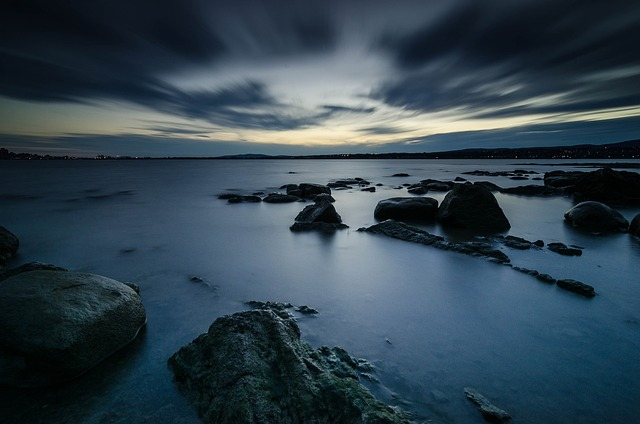
\includegraphics[width=0.75\textwidth]{image}
	\caption{some cool photo}
	\label{fig:image}
\end{figure}


\ref{fig:image} labeled figure reference.

\pageref{fig:image} page reference based on labeled figure

\begin{itemize}
	\item unordered item
	\item unordered item numero dos
\end{itemize}

\begin{enumerate}
	\item ordered list
	\item ordered list numero uno
\end{enumerate}

\textbf{Math Stuff}

In physics, the mass-energy equivalence is stated by the equation $E=mc^2$, discovered in 1905 by Albert Einstein.

\begin{math}
	E=mc^2
\end{math}

\[E=mc^2\]

\begin{equation}
	E=mc^2
\end{equation}

\begin{math}
	T^{i_1 i_2 \dots i_p}_{j_1 j_2 \dots j_q} = T(x^{i_1}, \dots, x^{i_p}, e_{j_1}, \dots, e_{j_q})
\end{math}

\vspace{5mm}

integral = $\int$, fraction = $\frac{a}{b}$.

Limits are placed on integrals using subscripts and subscripts:
\[ \int_0^1 \frac{dx}{e^x} = \frac{e-1}{e}\]

Lower case greek letters = $\omega$ $\delta$, uppercase = $\Omega$ $\Delta$

Mathemtical operators are prefixed with a backslash as $\sin(\beta)$, $\cos(\alpha)$, $\log(x)$ etc.

\section{Math}

\subsection{Math Mode Accents}

\begin{align*}
    \hat{a}&hat & \bar{a}&bar & \vec{a}&vec \\
\end{align*}

\begin{align*}
    \alpha && \beta && \gamma && \delta \\

\end{align*}


\end{document}
